\origpage{53}{GRAPH MINORS}
\noindent\hspace*{12pt}\textit{$e$ of $G_1$, if $e$ has ends $v, v'$ say, then $f(e)$ has one end in $Y(v)$ and the other
in $Y(v')$.}

\hspace*{12pt}(M4)\quad$\rho(G_2)\in Y(\rho(G_1))$.
\stmt
We now introduced two further classes of trees. If $\gamma\ge 1$, $\delta\ge 1$ are
integers, the rooted tree $P(\gamma, \delta)$ is defined as follows: Take $\delta$ disjoint copies
of $\mathbf{H}_{\gamma-1}$. Each of these copies has a unique vertex of even valency; let these
be $u_1,..., u_\delta$, say. Take a path of $\delta$ new vertices $v_1,..., v_\delta$ say, and for
$1\le i\le\delta$, add an edge joining $u_i$ and $v_i$. The resultant graph is rooted at $v_1$,
and is $P(\gamma, \delta)$. We also define $P(0, \delta)$ to be the path of $\delta$ vertices, rooted at
one end, for $\delta\ge 1$.

Second, if $\gamma\ge 1$, $\delta\ge 2$ are integers, we define a rooted tree $Q(\gamma, \delta)$ as
follows: Take a copy of $P(\gamma-1, \delta-1)$, with root $v_1$ say, and a disjoint copy
of $\mathbf{H}_{\gamma-1}$. Let $v_2$ be the (unique) vertex of the second graph with even valency.
Take a new vertex $v$, and two new edges, joining $v$ to $v_1, v_2$, respectively.
The resultant graph is $Q(\gamma, \delta)$, and it is rooted at $v$. (See Fig. 4.)

Now let $\lambda\ge 1$ be odd. Define $\theta=\max(6, 2^{(\lambda+3)/2})$, $\alpha=2^{\theta^4}$, and $\beta=2^{\theta^6}$.
For integers $x, i\ge 0$, define $f_i(x)$ inductively, by
\begin{equation*}
f_0(x)=x,\qquad f_i(x)=f_{i-1}(\beta^x)(i>0).
\end{equation*}
For integers $\gamma, \delta$ with $\gamma\ge 0$, and $\delta\ge 2$, define $p(\gamma, \delta)=f_\gamma(\delta)$; and if $\gamma\ge 1$,
define $q(\gamma, \delta)=f_{\gamma-1}(\beta+2\delta)$.
\stmt
(3.6). \textit{With the above definitions, the following inequalities hold}:

\hspace*{12pt}(i)\enspace $p(0, \delta)\ge\delta-2$ \textit{for all} $\delta\ge 2$;

\hspace*{12pt}(ii)\enspace $q(\gamma, \delta)\ge\theta^2+p(\gamma-1, 2+4\theta^{2\theta}+2\delta)$ \textit{for} $1\le\gamma$, $2\le\delta$;

\hspace*{12pt}(iii)\enspace $p(\gamma, \delta)\ge q(\gamma, 4)$ \textit{for} $1\le\gamma$, $2\le\delta$;

\hspace*{12pt}(iv)\enspace $p(\gamma, \delta)\ge\alpha^{\delta\cdot 2^\gamma}+\max(p(\gamma, \delta-1), q(\gamma, 3\alpha^{\delta\cdot 2^\gamma}+6))$ \textit{for} $1\le\gamma\le\lambda$,
$3\le\delta$.
\stmt
\textit{Proof}. This is routine\del{, and is left to the reader}. \fix{By definition,
$f_i(x)=f_{i-1}(\beta^x)$ for $i\ge 1$ and $x\ge 0$.

\hspace*{12pt}(1) \textit{For each integer $i\ge 0$, $f_i$ is strictly increasing, and
$f_i(x+d)\ge f_i(x)+d$ for all integers $x,d\ge 0$.}

The map $f_0$ is the identity. For $i>0$, $f_i$ is the map $x\mapsto\beta^x$ followed by
$f_{i-1}$. The first is strictly increasing since $\beta=2^{\theta^6}>1$, and so $f_i$ is strictly
increasing, by induction on $i$. A strictly increasing map from the non-negative integers to
themselves increases by at least $1$ from $x$ to $x+1$, and so by at least $d$ from $x$ to $x+d$.
This proves (1).

\hspace*{12pt}(2) $\beta\ge 16$, \textit{and} $\beta\ge\theta^2+2+4\theta^{2\theta}$.

Since $\theta\ge 6$, we have $\beta=2^{\theta^6}\ge 16$ and $\theta^6=\theta^2\theta^4\ge
3\theta^2\ge 2\theta^2+3$. Since $\theta\le 2^\theta$, we have $\theta^{2\theta}\le 2^{2\theta^2}$.
Since also $\theta^2\le\theta^{2\theta}$, it follows that
$\theta^2+2+4\theta^{2\theta}\le 8\theta^{2\theta}\le 2^{2\theta^2+3}\le 2^{\theta^6}=\beta$. This
proves (2).

Now (i) holds since $p(0,\delta)=\delta$. For (ii), let $y=2+4\theta^{2\theta}+2\delta$. By (2),
$\beta+2\delta\ge y+\theta^2$, and so by (1),
$q(\gamma,\delta)=f_{\gamma-1}(\beta+2\delta)\ge f_{\gamma-1}(y)+\theta^2=p(\gamma-1,y)+\theta^2$. For
(iii), $\beta^\delta\ge\beta^2\ge\beta+8$ by (2), and so
$p(\gamma,\delta)=f_{\gamma-1}(\beta^\delta)\ge f_{\gamma-1}(\beta+8)=q(\gamma,4)$. For (iv), let
$A=\alpha^{\delta\cdot 2^\gamma}$. Since $\gamma\le\lambda$ and $\theta\ge 2^{(\lambda+3)/2}$, we have
$\theta^2\ge 2^{\lambda+3}\ge 2^{\gamma+1}$. Since also $\delta\ge 2$, it follows that
$\delta\cdot 2^\gamma\theta^4\le\frac12\delta\theta^6\le(\delta-1)\theta^6$. Hence
$A\le 2^{(\delta-1)\theta^6}=\beta^{\delta-1}$. Also $\beta+12\le 2\beta^{\delta-1}$, and so by (2),
\begin{equation*}
\beta^\delta\ge 16\beta^{\delta-1}\ge\max(\beta^{\delta-1}+A,\;7A+\beta+12).
\end{equation*}
By (1) it follows that
$p(\gamma,\delta)=f_{\gamma-1}(\beta^\delta)\ge f_{\gamma-1}(\beta^{\delta-1})+A=p(\gamma,\delta-1)+A$,
and that
$p(\gamma,\delta)\ge f_{\gamma-1}(\beta+6A+12)+A=q(\gamma,3A+6)+A$. So $p(\gamma,\delta)$ is at least
$A$ plus the larger of $p(\gamma,\delta-1)$ and $q(\gamma,3A+6)$, and this proves (iv).\fixnote{fix:3.6-proof-added}{The paper leaves this proof to the reader. The argument above
is the one used in the formalization.}}
\stmt
The aim of the next two sections is to prove the following:

{\centering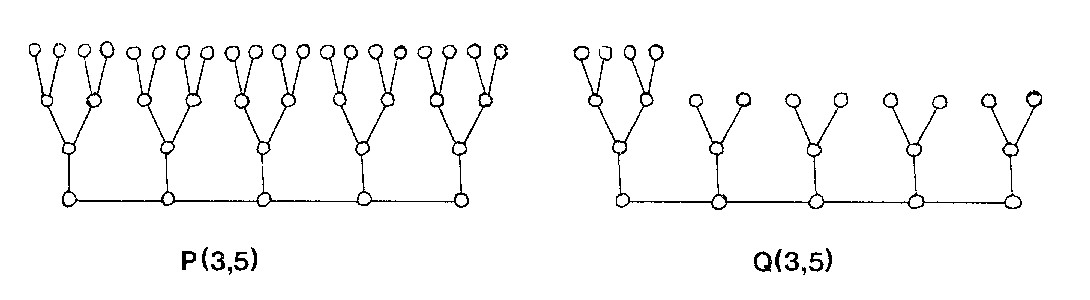
\includegraphics[width=262bp]{figures/fig4}\par
\vspace{12pt}{\small\textsc{Figure} 4}\par}
